\documentclass[english, 12pt, a4paper]{article}
\usepackage[utf8]{inputenc} 
\usepackage[T1]{fontenc,url} %url
\urlstyle{sf} %sf
\usepackage{babel,textcomp,csquotes, varioref,graphicx, gensymb}
% \usepackage[]{circuitikz}
\usepackage{tikz}
\usetikzlibrary{shapes,arrows}
\usepackage[backend=biber,style=numeric-comp, sortcites]{biblatex}

\title{INF4420 - Project description}
\author{Espen Klein Nilsen and\\
	Vegard Midtbøen}
\date{\today}

\begin{document}
 \maketitle
 
\section*{Introduction}
In this project we are going to design a Successive Approximation Register (SAR) Analog-to-Digital Converter (ADC). The project is a part 
of the cource INF-4420 at the University of Oslo, department of Informatics.\\
\\
The purpose of data converting is to interface the analog to the digital diomain, which is essential in almost every circuit.\\
\\
The SAR-ADC is buildt up by several modules, including sample-and-hold (S\&H), comparator and digital to analog converter. It is our task to design each of these modules, except the digital logic 
(the module is given by the cource instructor) for the system. The project covers all aspects of designing and implementing the SAR-ADC system, going from schematics to a circuit implemented in 
CMOS technology. There are given some minimum requirements that we must meet. The different modules of the system is to be simulated in Virtuoso by Cadence (schematics) and later simulated in layout. 
The parasitics is also going to be included in the simulation in Virtuoso.\\
\\
Since we are creating layout we must also make the circuit comply with the schematics by running Layout-vs-Schematics (LVS), Design-rule-check (DRC) and antenna tests. 
There are several other considerations in order to make a good layout. The task is therefore to identify theese challenges and find solutions to mitigate the situation. 
There are also several noise sources in the system whitch must be handled.\\
\\
The system consists of sevral parts, mainly:
\begin{itemize}
 \item Sample \& hold
 \item Comparator
 \item Digital to Analog Converter
 \item Digital SAR logic
\end{itemize}
The task is given in such a way that we are free to choose the implementation of the different modules as long as it meet the requirements. 
We must therefore research circuits that can perform these tasks and meet the specifications. 

\section*{Project plan}
The assignment is divided into subtasks where the different parts of the design, is to be designed.\\
\\
The order is: 
\begin{itemize}
 \item Design testbench
 \item DAC design
 \item Implementation of S\&H, Comparator and SAR logic
 \item Implementation of DAC into SAR-ADC
\end{itemize}
We assume that we are supposed to create and simulate schematics (etc.) and create layout for each task consecutively (as opposed to first creating all the schematics and then all layout).\\
\\
The final deadline is: 09.05.2016, 5pm.

\section*{Execution}
\subsection*{Task1: Design testbench}
The purpose of this task is to create a simulation enviroment for testing our solution. This setup should encourage testdriven development so we can spot implementation flaws early.
In this testbench we want to identify correctnes and performance (and limitations and stability).\\
\\
To create a suitable test enviroment we are going to create multiple (\textit{simple}) test benches to test the different modules.
We are also going to create a high-level testbench to simulate the complete system. The overall block diagram is shown in Figure \ref{block_diagram}. 
For a test input of 0.5V we expect a behavior as depicted in the waveform-drawing in Figure \ref{timing}.\\
\\
\tikzstyle{block} = [draw, fill=blue!20, rectangle, 
    minimum height=4em, minimum width=3em]
\tikzstyle{input} = [coordinate]
\tikzstyle{output} = [coordinate]
\tikzstyle{pinstyle} = [pin edge={to-,thin,black}]
% The block diagram code is probably more verbose than necessary
\begin{figure}
  \begin{tikzpicture}[auto, node distance=2cm,>=latex']
      % We start by placing the blocks
      \node [input, name=input] {};
      \node [block, right of=input, node distance=2cm] (sample_and_hold) {S\&H};
      \node [block, right of=sample_and_hold, node distance=4cm] (comparator) {Comparator};
      \node [block, right of=comparator, node distance=4cm] (sar_logic) {SAR Logic};
      
      % We draw an edge between the controller and system block to 
      % calculate the coordinate xsh(t). We need it to place the measurement block. 
      \draw [->] (sample_and_hold) -- node[name=xsh(t)] {$x_{sh}(t)$} (comparator);
      \draw [->] (comparator) -- node[name=xc(nT)] {$x_{c}(nT)$} (sar_logic);
      \node [block, below of=sar_logic, node distance=3cm] (dac){DAC};
      \node [output, right of=sar_logic, node distance=3cm] (output) {};
    
      % Once the nodes are placed, connecting them is easy. 
      \draw [draw,->] (input) -- node [name=xc(t)] {$x_{c}(t)$}(sample_and_hold);
      \draw [->] (sar_logic) -- node [name=digital_out] {Digital out}(output);
      \draw [->] (sar_logic) -- node [name=nbit] {N-bit} (dac);
      \draw [->] (dac) -| node [name=negfeedback, bend left] {Negative feedback}(comparator);     
  \end{tikzpicture}
  \caption{Block diagram}
  \label{block_diagram}
\end{figure}
The SAR ADC architecture is compared with three other architectures, as seen in Table \ref{comp:adc}.
\begin{table}[!ht]
\centering

\begin{tabular}{|l|l|l|l|l|}
\hline
                 & SAR        & Flash   & Sigma-Delta  & Integrating                      \\ \hline
Conversion speed & Low-medium & Fast    & Low          & Depending on 			  \\ 
		 &	      &		&	       & resolution and			  \\
		 &	      &		&	       & clock				  \\ \hline
Sampling rate    & Nyquist    & Nyquist & Oversampling & Nyquist                          \\ \hline
Area             & Low        & High    & Medium       & Low                              \\ \hline
\end{tabular}
\caption{Comparation of different ADCs}
\label{comp:adc}
\end{table}

\subsection*{Task2: DAC design}
In this task, we will study different DAC designs and make a schematic in Cadence. When designing DACs, there are several importaint specifications that needs to be considered. It is
our task to identify different specifications to fit with our requirements.

\subsection*{Task3: S\&H, Comparator, SAR logic}
There are many different approces to create S\&H, comparator and SAR logic. Also here we need to investigate different designes.


\subsection*{Task4: Implementation of DAC into SAR-ADC}
In this task the DAC is to be integrated into the SAR system. 

\begin{figure}[!ht]
  \centering
    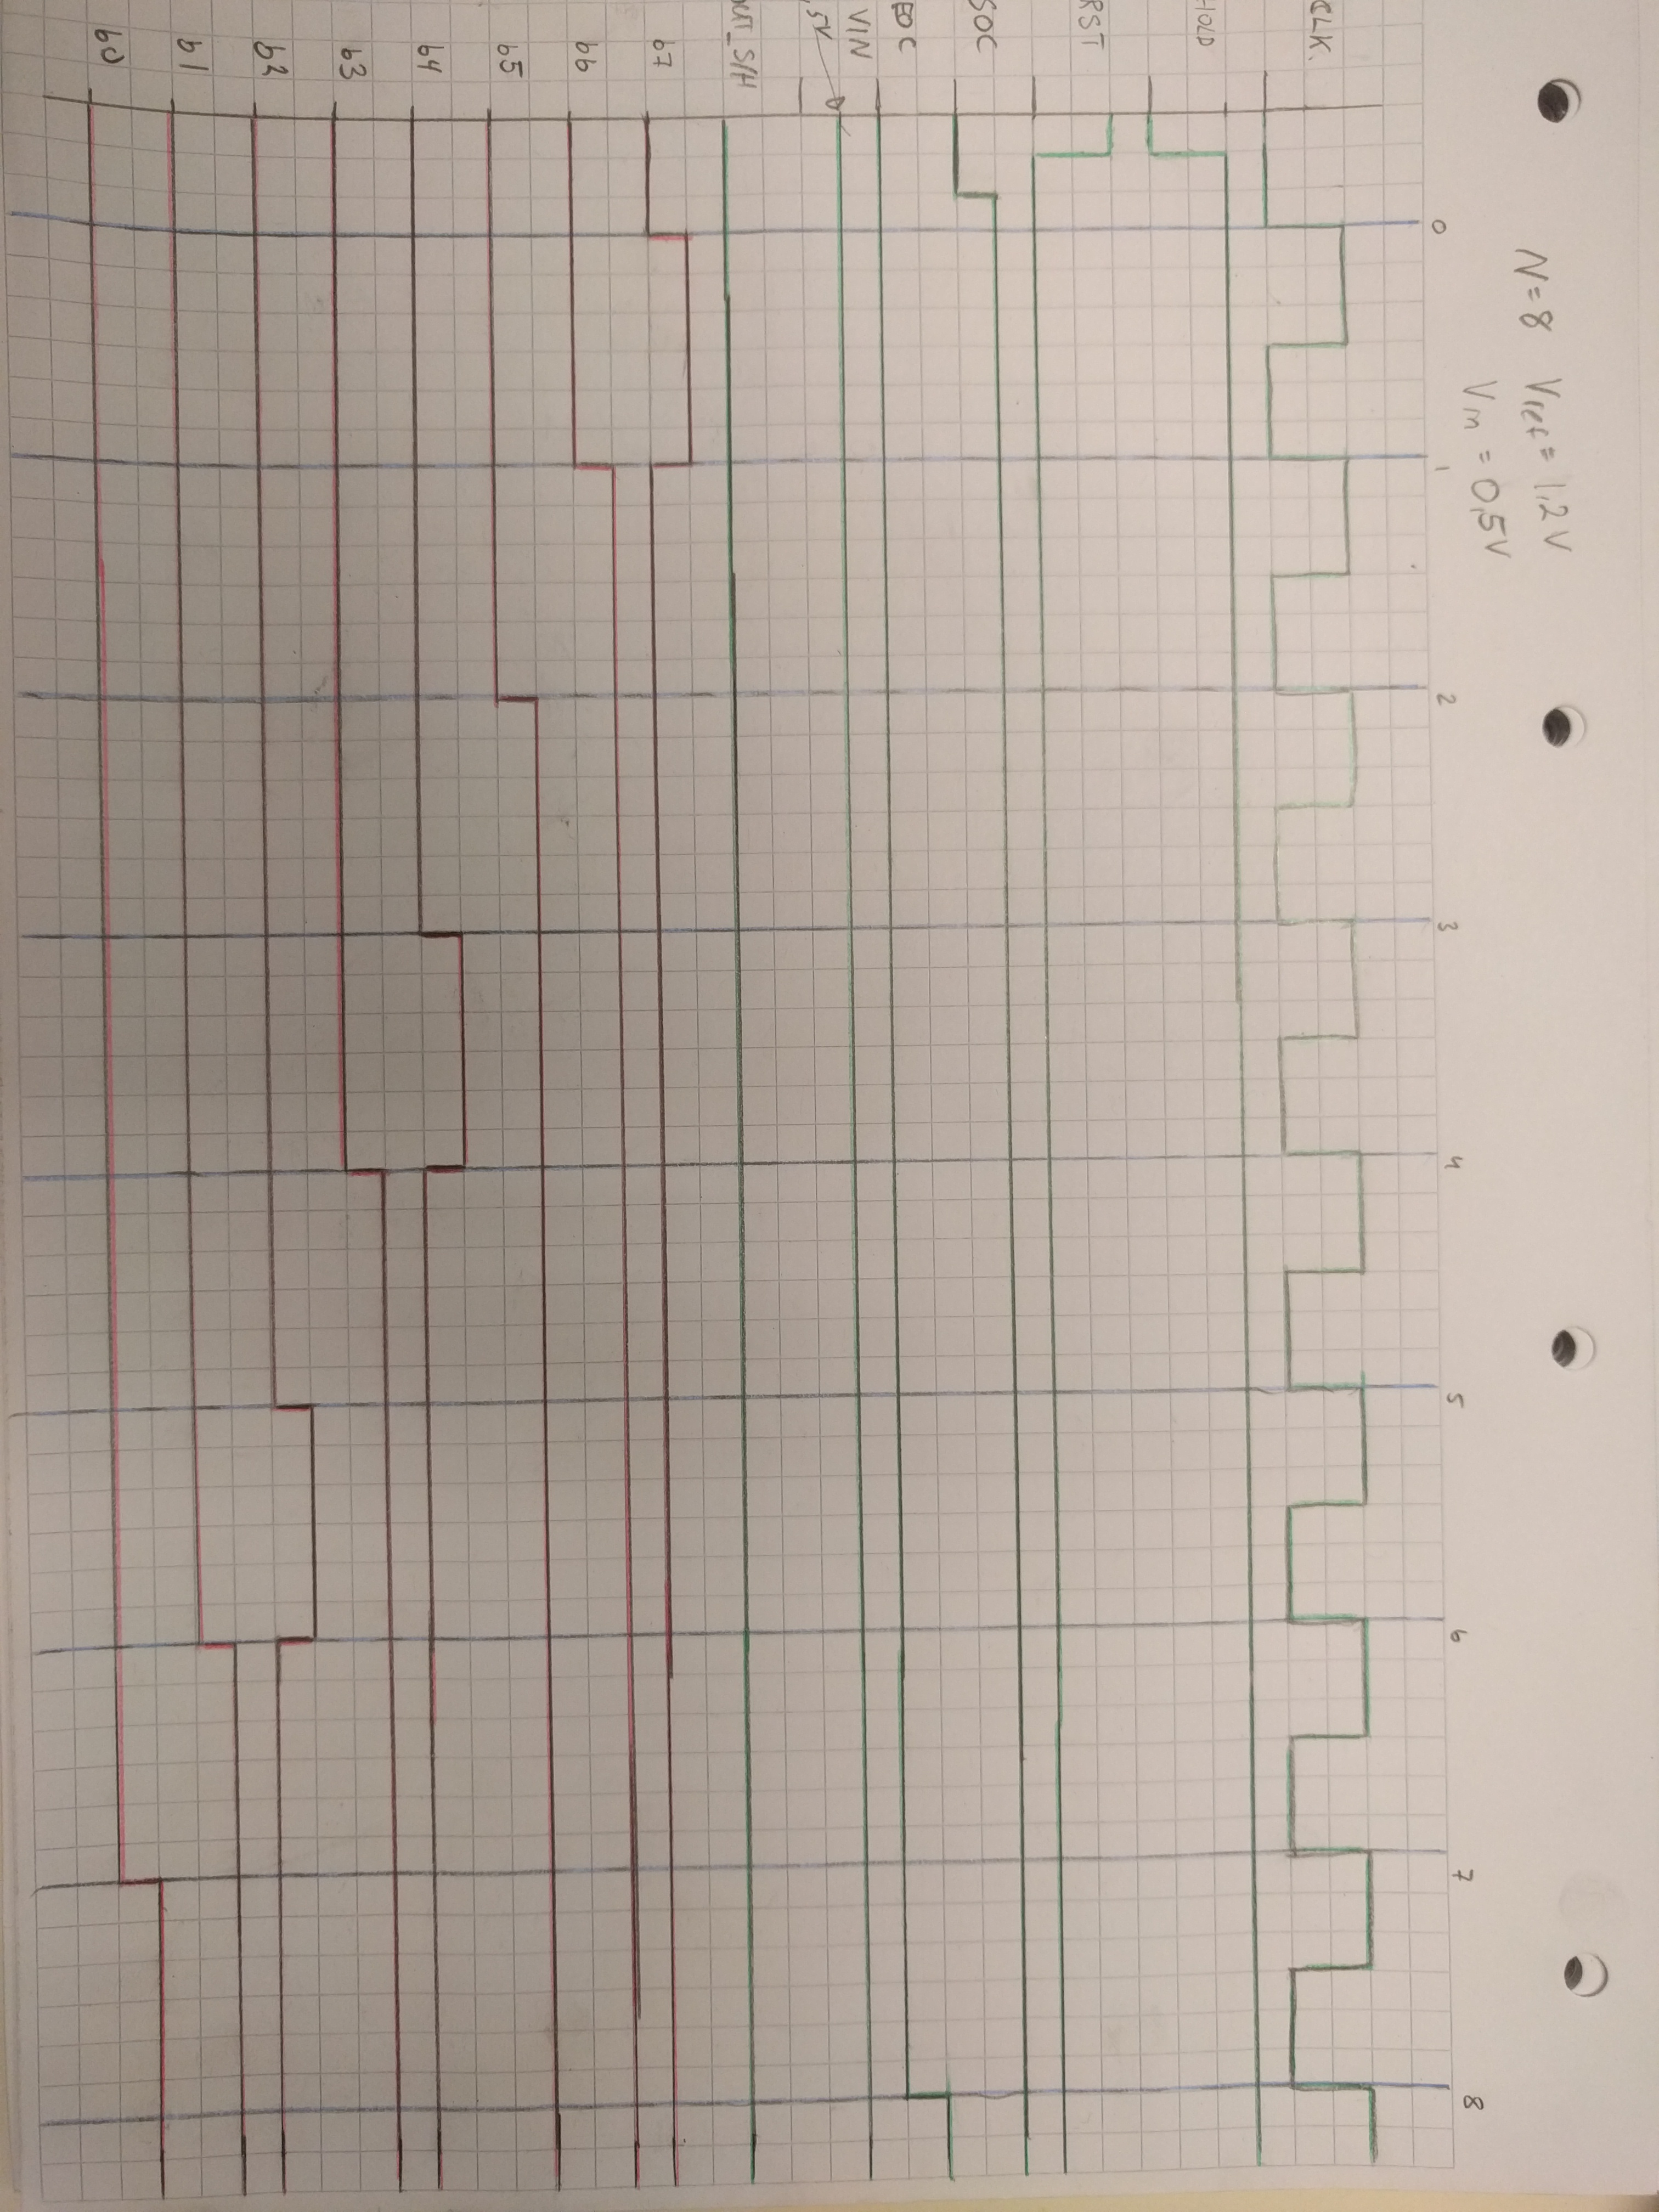
\includegraphics[width=0.8\textwidth]{timing_diagram_color.jpg}
    \caption{Timing diagram}
    \label{timing}
\end{figure}

\end{document}
